% \chapter{I PARTE}

INSERISCI GLI EXCURSUS IN FORMA DI APPENDICI

\chapter{Accrescimento e dischi - ch. 1 e 5 King}

% \section{Two bodies problem without lagrangian approach}
% 
% \subsection{Problem delineation}
% 
% \subsubsection{Reduction to a one body problem}
% The two bodies problem is equivalent to a single body of reduced mass $\mu = \frac{M_1  M_2}{M_1+M_2}$ relative acceleration $a_{acc} = a_{acc, 1} - a_{acc,2} $, orbiting around a fixed center of force generated by a field $-\frac{GM}{r^2} = -\frac{G(M_1+M_2)}{(r_1+r_2)^2} $, where
% \begin{itemize}
%     \item $r=r_1+r_2 $
%     \item $M = M_1+M_2 $
%     \item $r_1= \frac{M_2}{M}r $
%     \item $r_2= \frac{M_1}{M}r $
% \end{itemize}
% 
% \subsubsection{Symmetry implies Angular Momentum conservation $L$ end planar orbits}
% \subsubsection{The trajectories are ellipses}
% In polar coordinates:
% \begin{equation}
%     r = \frac{a(1-e^2)}{1+e\cos{\theta}},
% \end{equation}
% where $(\frac{a}{b})^2 = 1-e^2 $, $S = area = \pi ab$, and $a,b$ are the ellipse's semiaxes.
% 
% \subsection{Theorems}
% 
% \subsubsection{I Theorem}
% The angular momentum is proportional to the orbit area
% 
% \subsubsection{II Theorem (III Kepler's law)}
% 
% \subsubsection{}

\section{Two bodies problem without lagrangian approach}
Energie e momenti angolari in sistema binario, leggi di Keplero e teoremi vari, potenziale efficace. Vedi dai suoi appunti.

\section{Accrescimento}

\subsection{Energia e momento angolare}
Il disco che si viene a formare è una struttura \textbf{stazionaria} (ma non statica), nella quale $v_{rad}<<v_{tang} $; per questo motivo, vale il \textbf{teorema del viriale}:
\begin{equation}
    E_{tot} = U + K = -\frac{1}{2}\frac{GMm}{r}.
\end{equation}
A causa di questo, particelle di materia appartenenti a raggi vicini perdono energia, e di conseguenza cadono, la loro energia potenziale diventa sempre più negativa e quella cinetica sempre più grande, cioè accelerano: la viscosità le frena, e quando cadono riaccelerano.
Come si è visto negli appunti "Two bodies problem without lagrangian approach", $L\propto S \Omega = \pi r^2 \Omega$ per orbita circolare, quindi:
\begin{align}
    &v_A = \frac{dS}{dt} = \frac{A_{orb}}{T}, quindi\notag\\ 
    &L = mr\times v = mr\times |r|\Omega\notag\\
    &= mr^2\Omega =mr^2\sqrt{\frac{GM}{r^3}} \propto \sqrt{r}.
\end{align}
Ne consegue che, per $r\xrightarrow{} 0$, il momento angolare diminuisce e $E_{tot}$ sarà sempre più negativa: metà dell'energia la manterrà, metà la perderà, emettendola.

\subsubsection{Sulla radiazione emessa dal disco}
Il disco presenta regioni a temperature diverse lungo il suo raggio. 
Ne consegue che lo spettro di corpo nero emesso sarà più freddo fuori e più caldo dentro, e quello misurato sarà una somma di questi contributi.
Inoltre, è importante notare che individualmente i fotoni si portano via momento angolare, in unità intere pari a $\pm 1$.
Nei fotoni polarizzati circolarmente, infatti, i campi non oscillano, ma \textit{ruotano}, come la somma di moti oscillatori coordinati lungo direzioni $x$ e $y$.
\begin{figure}[h!]
    \centering
    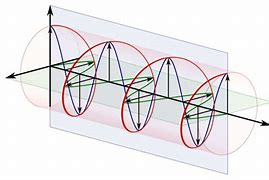
\includegraphics[width=0.5\linewidth]{Immagini/circular_polarization.jpeg}
    %\caption{}
    \label{fig:enter-label}
\end{figure}
Poiché i fotoni vengono emessi in ogni direzione, e casualmente con polarizzazione destra e sinistra, nel complesso il momento angolare totale che porteranno via dal disco sarà 0\footnote{Esistono in effetti casi astrofisici in cui il momento angolare può essere perso tramite la radiazione emessa. Ad esempio questo avviene nelle pulsar, che ruotando emettono radiazione: in questo caso si tratta di un'emissione non termica, coerente (come si vedrà più avanti).}.
\subsubsection{Il tragitto del momento angolare}
Abbiamo visto che il momento angolare diminuisce, ma che non può essere a causa della radiazione emessa. 
Questo significa che l'unica cosa che può fare è trasferirsi lungo il disco, verso l'esterno, attraverso la materia in caduta:
il disco, in questo modo porta materia verso l'interno, e momento angolare verso fuori.
La parte più esterna del disco in questo modo accumulerà momento angolare, e dovrà quindi aumentare di raggio fino a staccarsi.
A causa delle forze mareali, la stella compagna attira il disco, formandovi una protuberanza, che a causa della rotazione del disco sarà sempre un po' oltre la linea che congiunge i due corpi: la rotazione tenderà ad allontanarla, mentre la gravità tirerà per riallinearla.
Questo processo genera una forza di taglio gravitazionale che, frenando la protuberanza che ruota via, genera un momento torcente attraverso il quale il momento angolare viene perso dal disco, e recuperato dalla compagna. 
\subsubsection{Momento angolare per unità di massa}
Se si considera il momento angolare per unità di massa, definito come
\begin{equation}
    \vec{l} = \frac{\vec{L}}{\mu} = \sqrt{G(M_1+M_2)r}
\end{equation}
di un pezzetto di materia di massa $M_2=m << M_{ns}=M_1$ in orbita attorno a una stella di neutroni a una certa distanza $a/2$, questo sarà
\begin{equation}
    \vec{l}_m = \frac{L_m}{\mu}\simeq \sqrt{GM_{ns}\frac{a}{2}}.
\end{equation}
Per una stella compagna, di massa $M_2 = M_{comp} \sim M_{ns} = M_1 $, che orbiti a una distanza doppia, pari a $a$, sarà invece
\begin{equation}
    \vec{l}_{comp} = \frac{L_{comp}}{\mu} \simeq \sqrt{2GM_{ns}a}.
\end{equation}
In pratica, il momento angolare per unità di massa di un pezzetto di massa $m$ che sta in orbita, e quello della stella compagna che orbita a distanza simile, sono molto simili: 
la stella compagna cede massa alla NS, ma il momento angolare gli torna indietro. Poiché però sta perdendo massa, $M_{comp}$ diminuisce, e quindi diminuisce anche $l_{comp} = \sqrt{G(M_1+M_2)r} $, e 1si trova per questo motivo a doversi allontanare: $L_{comp} $ resta costante, mentre $l_{comp} $ no.
A tutti gli effetti del momento angolare, l'accrescimento è come se avvenisse radialmente.

IN QUESTA PARTE NON SI CAPISCE BENE DAGLI APPUNTI, INTEGRA SE POSSIBILE E CORREGGI IL RAGIONAMENTO.

\subsubsection{Energia}
A differenza del momento angolare, che è un vettore, l'energia è una quantità scalare, e quindi somma sempre positivamente.
Se mi interessa quanta energia ho rilasciato, posso definire il potenziale fregandomene del percorso:
\begin{equation}
    U(r) = -\frac{GM}{r}.
\end{equation}
Se la materia che accresce parte da un raggio grande $a$, e arriva a un raggio $\sim0$, 
\begin{align}
    \Delta U = U_f-U_i = -\frac{GM}{r_f} + \frac{GM}{r_i} \\
    = -\frac{GM}{r_f}[1 - \frac{r_f}{r_i}] \simeq -\frac{GM}{r_f}.
\end{align}
Di conseguenza, l'energia che la radiazione può portarsi dietro sarà
\begin{equation}
    \Delta E_{acc} = \frac{GM}{R}m,
\end{equation}
e quindi
\begin{equation}
    \boxed{L_{acc} = \frac{\Delta E_{acc}}{\Delta T} = \frac{GM}{R}\frac{m}{\Delta T} = \frac{GM}{R}\dot{M}}\hspace{1mm}.
\end{equation}
Inoltre, notando che $\Delta E_{acc} = \frac{GM}{R}m_0 =\epsilon m_0 c^2$, si definisce l'\textbf{efficienza dell'accrescimento} come
\begin{equation}
   \epsilon_{acc} = \frac{GM}{Rc^2} = \frac{2GM}{c^2}\frac{1}{2R} = \frac{R_{schw}}{2R} \le \frac{1}{2},
\end{equation}
dal momento che $R_{schw} \le R$: cioè tramite accrescimento, per un buco nero di Schwarzschild ($R=R_{schw}$) si può bruciare fino a metà della massa di riposo $m_0$\footnote{Per buchi neri rotanti di Kerr, $R_{schw_{Kerr}} = \frac{1}{2}R_{schw} $, quindi $\epsilon_{acc_{Kerr}}\le 1 $}.

\subsubsection{Circolarizzazione}
Abbiamo visto come nell'accrescimento, il sistema perde energia lasciando invariato il momento angolare. Come sappiamo, l'orbita che, a parità di momento angolare, ha il minimo valore di energia, è l'orbita circolare: tramite questo processo, l'orbita tenderà a \textit{circolarizzare}. 
Si noti che circolarizzando $r$ diminuirà, e quindi $l = \sqrt{GMr} =\frac{L}{m}$ diminuirà.
Infatti, orbite circolari sempre più vicine perdono momento angolare, mentre ciò non è vero per orbite ellittiche, dove i semiassi $a$ e $b$ possono variare compensandosi.
Alla fine, una volta raggiunta l'orbita circolare, l'attrito viscoso rallenta la materia, che tenderà a scendere nel disco e, poiché l'orbita a questo punto è circolare, il sistema perderà proprio momento angolare $L$ (che viene quindi trasferito verso l'esterno o sulla stella primaria tramite la materia accresciuta, come vedremo meglio più avanti)\footnote{Vedasi Appendice B: tempo di caduta dalla luna usando un'orbita ellittica.}.


\subsubsection{Sulle efficienze}
A questo punto, è utile confrontare l'efficienza del processo di accrescimento con altri processi di produzione di energia\footnote{Vedasi Appendice C per digressione sulle esplosioni}.
Sappiamo, ad esempio, che l'efficienza del processo di fusione nucleare, maggiore rispetto a quella del processo di fissione, è data da $\frac{m ^4_2He}{4m_p} = 0.006 \simeq 10^{-2} $.
L'energia di un legame chimico, d'altra parte, è circa pari a $E_{ion,H} = 13.6eV $, e quindi l'efficienza risulta pari a $\epsilon_{chim} = \frac{13.6eV}{m_p} \sim 10^{-8} $.\\
Confrontiamo questi risultati con alcuni esempi di accrescimento:
\begin{itemize}
    \item Terra: $R_{Schw,\oplus} = \frac{1}{300000}R_{schw,\odot} \simeq 1cm \xrightarrow{}  \epsilon_{acc,\oplus} \simeq 5\times10^{-10} $, bassissimo;
    \item Sole: $\epsilon_{acc,\odot} = 2\times10^{-6}>\epsilon_{chim} $, e già si migliora;
    \item Nana bianca: $R_{wd}\sim 10^{9} \xrightarrow{} \epsilon_{wd}\sim 10^{-4} $;
    \item Stella di neutroni:  $R_{NS}\sim 10^{6} \xrightarrow{} \epsilon_{NS}\sim 10^{-1} $!!
\end{itemize}
L'accrescimento su oggetti compatti, è uno dei processi più energetici dell'universo: i più energetici dopo il Big Bang.
Si noti che, per accrescimento radiale su un BH, l'efficienza è nulla: il buco nero si mangia tutta l'energia, e manca la superficie su cui sbattere e rilasciare l'energia.
Se in caduta libera tutta l'energia potenziale si trasforma in energia cinetica, il fatto che un disco sia un sistema virializzato, comporta che solo metà dell'energia potenziale possa essere trasformata in cinetica, mentre l'altra metà può essere emessa. Questo fatto introduce un nuovo fattore $\frac{1}{2}$, per cui in realtà
\begin{equation}
    \epsilon_{acc_{disco}} = \frac{1}{4}\frac{R_{schw}}{R} \le 0.25 \hspace{1mm} .
\end{equation}\\
COMPLETA QUESTA PARTE CON CH. 1 DEL LIBRO.

\subsubsection{Dischi di accrescimento: perché si formano?}

Si immagini di cercare di far cadere una particella su un buco nero da una distanza di $1AU$: questo sottenderà un arco di $\sim \frac{10^5}{10^{13}} rad= 10^{-8} rad$, per cui avrei bisogno di una precisione di almeno $10^{-9}rad$.
Ora, in $2\pi \hspace{1mm}rad$ ci sono $3600arcsec$, quindi in $10^{-9}rad $ ci sono $\sim 10^{-6}arcsec$ circa: ci vuole una precisione impressionante.
Infatti, in genere le cose non cadono radialmente, ma mancano il bersaglio, e seguono ellissi più o meno elongate. Nella pratica, l'accrescimento radiale sferico non avviene praticamente mai.




\section{Sui potenziali gravitazionali}

\subsection{Lezione sui BH, perché si - ch. 1 Taylor, Wheeler - ch. 1 Shultz (vedi drive) - Forse andrebbe in Appendice?}
Come sappiamo, Schwarzschild ricavò, nell'ambito della relatività generale, la metrica deformata da un buco nero non rotante e non carico, come
\begin{equation}
    ds^2 = c^2dt^2\left( 1-\frac{R_{sch}}{r} \right) - dr^2 \left( 1-\frac{R_{sch}}{r} \right)^{-1}-r^2\sin^2{\theta}d\phi^2-r^2d\theta^2,
\end{equation}
che per un moto radiale ($d\theta=d\phi=0 $) diventa
\begin{equation}
    ds^2 = c^2dt^2\left( 1-\frac{R_{sch}}{r} \right) - dr^2 \left( 1-\frac{R_{sch}}{r} \right)^{-1},
\end{equation}
dove $dt$ è il tempo misurato da un osservatore a distanza infinita dal BH (stesso vale per $dr$).
Invece, per un osservatore che si pone fermo ($dr=0 $) ad un raggio fissato a un pelo fuori dal BH, $r=R_{sch}+\epsilon $, il tempo che misurerà sarà 
\begin{equation}
    d\tau^2 = c^2dt^2\left( 1-\frac{R_{sch}}{R_{sch}+\rho} \right) = c^2dt^2\left( 1-\frac{1}{1+\epsilon} \right) \simeq c^2dt^2\epsilon,
\end{equation}
dove abbiamo definito $\rho = \epsilon R_{sch} $ l'incremento infinitesimo \textit{dimensionale} ($\epsilon $ è \textit{adimensionale}), e abbiamo usato il fatto che $(1+\epsilon)^{-1} \sim 1-\epsilon $.
Se per un osservatore vicino passa un tempo finito $d\tau$, per un osservatore a infinito passerà dunque $dt=\frac{d\tau}{\sqrt{\epsilon}}\xrightarrow{\epsilon\xrightarrow{}0}\infty $.
\subsubsection{Un buco allo stomaco? O nella teoria?}
Può a questo punto sorgere un dubbio concettuale: dalla Terra osserviamo buchi neri di ogni taglia, e sappiamo che quelli più grossi lo sono diventati "mangiando" enormi quantità di materia.
Dal nostro punto di vista, della materia che cade in uno di questi buchi neri dovrà impiegare un tempo infinito a superare l'orizzonte degli eventi (il tempo diventa grande quando $\epsilon $ diventa piccolo, e siamo in buona approssimazione a distanza "infinita" da essi): come facciamo allora ad osservare buchi neri che, di materia, ne hanno mangiata eccome, e in tempi (necessariamente) almeno inferiori alla vita dell'universo?
In altre parole, come facciamo a "osservare" i buchi neri crescere se, dal nostro punto di vista, non mangeranno mai, anche in un tempo infinito, della materia? E il buco nero stesso, come fa dal suo punto di vista a crescere di massa?
Per dare una risposta qualitativa, consideriamo un oggetto sferico di densità uniforme e costante $\rho_0 $, che avrà di conseguenza una massa $M = \frac{4}{3}\pi R^3 \rho_0$. Il suo raggio crescerà, al crescere della massa, come $R\propto M^{1/3}\rho_0^{1/3} $. 
Sappiamo d'altronde che il raggio di Schwarzschild di un oggetto di massa M, per definizione, va come $R_{sch} \propto M $: se l'oggetto ha una densità fissata $\rho_0$, finché $M<M^*$ ($M^*$ la massa per cui $R=R_{sch}$) non collasserà.\\
\begin{figure}[h!]
    \centering
    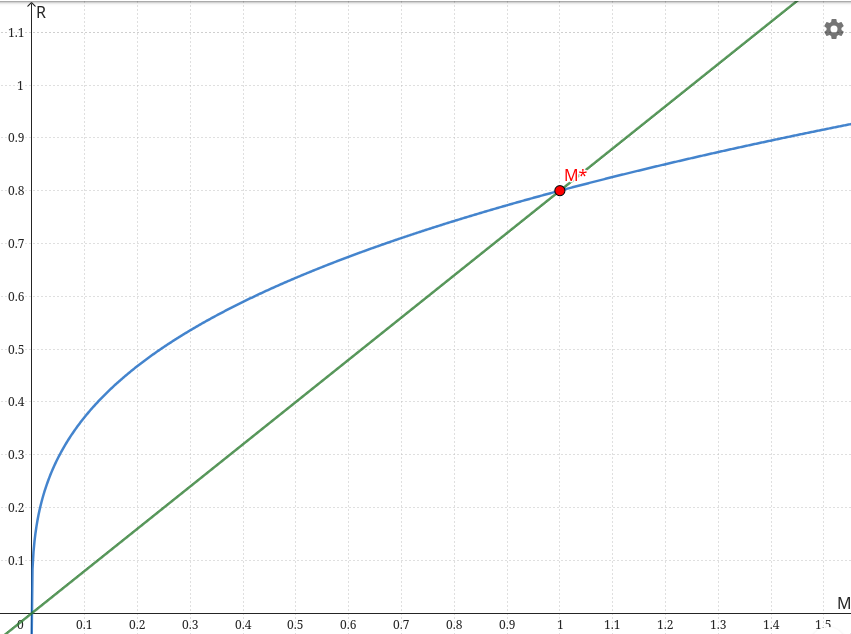
\includegraphics[width=0.7\linewidth]{Immagini/collasso_out_in_grafico.png}
    %\caption{}
    \label{fig:enter-label}
\end{figure}

Immaginiamo ora di depositare, sulla superficie dell'oggetto sferico isodenso una nuova shell di massa a densità $\rho_0$:
se la massa è ancora inferiore a $M^*$, l'oggetto non è un BH e non ho problemi a vederlo crescere; se invece $M>M^*$, l'oggetto è un BH, e dal grafico si vede che il $R_{sch}$ cresce più velocemente di $R$, e quindi l'orizzonte ingloba questa nuova massa crescendo più velocemente (e quindi oltre) del raggio dell'oggetto: il collasso è un processo \textbf{out-in}.

\subsection{Potenziale di Paczinsky-Wiita}
Il \textit{campo} è, in sostanza, una forza per unità di carica, dove la carica nel caso gravitazionale corrisponde alla massa.
Si capisce, da questa definizione, che nella GR il concetto stesso di \textit{campo gravitazionale} è fuorviante, e proprio sbagliato: la gravità NON è una forza, ma una manifestazione della deformazione dello spazio-tempo.
Attraverso una trattazione semi-classica, tuttavia, ci si può esprimere, per comodità, in termini di potenziali.
In particolare, per buchi neri non rotanti esiste un'approssimazione molto potente, nota come potenziale di Paczinsky-Wiita, che tiene conto della fenomenologia dei buchi neri.
Ad esempio, tramite il potenziale gravitazionale classico di Newton,
\begin{equation}
    U_N = \frac{GMm}{r} \xrightarrow{} F_N=-\frac{GMm}{r^2}, 
\end{equation}
si vede che la forza diventerebbe infinita per $r\xrightarrow{}0$, in corrispondenza di quella che in un BH prende il nome di \textit{singolarità}.
Tuttavia, proviamo a ragionare in termini di forze:
proviamo a immaginare di calare, con una canna da pesca dalla lenza inestensibile e infinitamente resistente, una particella di materia verso un buco nero, a partire da una distanza approssimativamente infinita.
La forza che servirà per trattenere, istante per istante, la particella dal cadere nel buco nero aumenterà sempre di più, come $\frac{1}{r^2}$, avvicinandosi al BH. 
Ma facciamoci caso: quand'è che la forza diventerà infinita? In altre parole, quand'è che davvero niente può essere più trattenuto dal cadere verso la singolarità? 
Nel momento in cui superiamo l'orizzonte degli eventi! È lì che niente può più sfuggire, neanche la luce, ed è lì che la forza per trattenere o tirare fuori della materia con questa canna da pesca divergerà.
Da questa semplice, ma importante intuizione, l'idea: possiamo descrivere un BH con un potenziale classico, attraverso una semplice correzione al denominatore del potenziale Newtoniano:
\begin{equation}
    U_{PW} = -\frac{GMm}{r-r_{sch}}.
\end{equation}
In questo modo la forza diverge effettivamente al raggio dell'orizzonte degli eventi.
Ricordiamo che, ovviamente, si tratta di un'approssimazione: la gravità in realtà non è una forza, e questo discorso vale solo per $m<<M$.
Tuttavia, per descrivere i dischi di accrescimento, va benissimo.

\subsubsection{Efficacia del metodo}
Testiamo ora questa approssimazione con alcuni problemi di GR.
Ad esempio, sappiamo che in GR il \textit{problema a due corpi} non è affatto banale: 
la "forza" che attrae il corpo 1 al corpo 2 dipende da una distanza (dal centro del corpo 1 all'orizzonte degli eventi del corpo 2, a una distanza $r_{sch,2}$ dal proprio centro) che è diversa dalla distanza dalla quale dipende la forza che attrae il corpo 2 al corpo 1 (il viceversa, con però un $r_{sch,1} \not= r_{sch,2}$), e quindi non posso ridurre il sistema a un solo corpo come fatto in meccanica Newtoniana.
Proviamo ad approcciare questo problema con questa approssimazione, per $m<<M$.
Descriviamo per prima cosa la forza centrifuga percepita dalla massa attraverso uno \textit{pseudo-potenziale} centrifugo, che dipende dal momento angolare (e quindi dalla velocità, da cui il "pseudo") della particella, che si conserva:
\begin{equation}
    F_c=\frac{mv^2}{r}=\frac{m^2v^2r^2}{mr^3} = \frac{L^2}{mr^3} = -\frac{\partial U_c}{\partial r}.
\end{equation}
A questo punto, calcoliamo il potenziale:
\begin{align}
    \int F_c dr = -\frac{1}{2}\frac{L^2}{mr^2}{\Big|}_{r_i}^{r_f}\\ 
    = -(U_{c,f} - U&_{c,i}) = -\frac{L^2}{2m}\left( \frac{1}{r_f^2} - \frac{1}{r_i^2} \right), 
\end{align}
e se mandiamo $r_f\xrightarrow{} \infty$ per $L$ fissato,
%, se aumenta $r$ diminuisce la velocità angolare.
\begin{equation}
    U_c = \frac{1}{r^2}\frac{L^2}{2m}.
\end{equation}
Il potenziale totale percepito dalla particella, quindi, sarà:
\begin{equation}
    U_{tot} = U_{PW} + U_c,
\end{equation}
e avrà la forma mostrata in \textbf{Figura \ref{fig:pw potential}}.
\begin{figure}[h!]
    \centering
    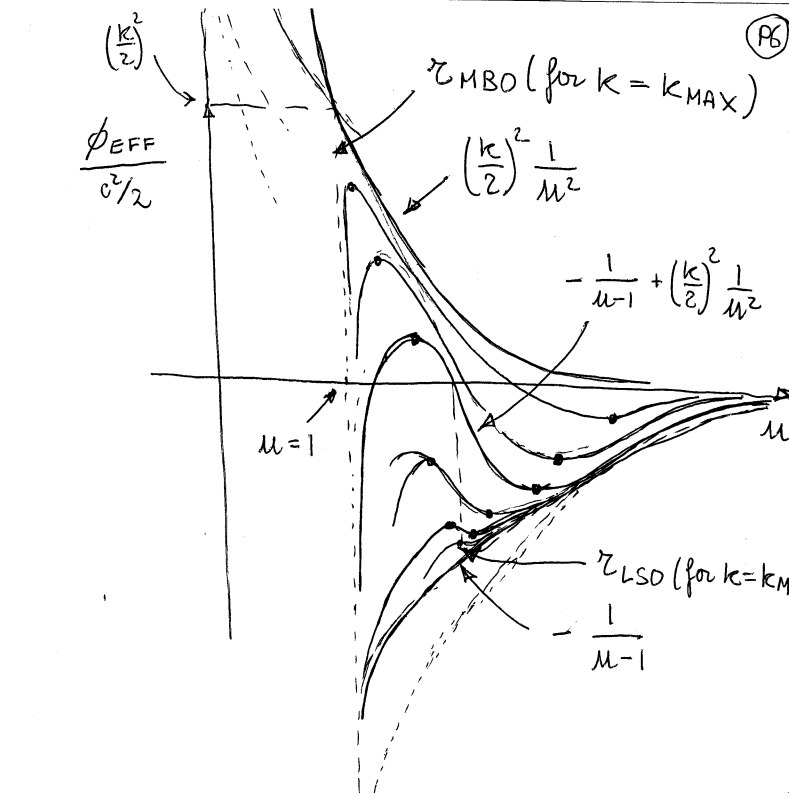
\includegraphics[width=0.7\linewidth]{Immagini/potenziale_PW.png}
    \caption{Rappresentazione del potenziale di PW, in cui a ogni curva corrisponde un diverso valore di momento angolare. Si vede che per $k$, e quindi $L$ più piccoli si tende ad abbassare il picco, e a spostarsi verso destra (il raggio di massimo avvicinamento stabile diventa più grande), fino a coincidere al limite con la valle, che corrisponde all'orbita circolare.}
    \label{fig:pw potential}
\end{figure}
Nell'immagine, le diverse curve corrispondono a valori diversi di momento angolare. 
I punti segnati nelle valli corrispondono a orbite circolari.
Se nel caso classico a parità di L aumenta l'energia, si incontrerà un asintoto verticale a sinistra, che respingerà sempre\footnote{In effetti, senza la correzione a denominatore, il potenziale gravitazionale diverge verso $-\infty$ come $1/r$ per $r\xrightarrow{}0$, proprio dove invece quello centrifugo diverge verso $+\infty$ come $1/r^2$: la correzione di PW invece sposta la divergenza negativa del potenziale gravitazionale più avanti, a un valore di $r$ corrispondente al raggio di Schwarzschild, e in quel punto il potenziale centrifugo è ancora limitato, e quindi viene sprofondato dalla divergenza di quello gravitazionale.}; nel caso relativistico di PW invece, avvicinandosi a $r_{sch}$ a un certo punto si supera un massimo, dopo il quale non si può più uscire, e si cade in una buca infinita.
Si noti che, per $L$ fissato, se aumenta $E$ aumenta anche la velocità radiale (se aumentasse quella tangenziale, cambierebbe $L$).
Calcoliamo ora il potenziale rappresentato in figura, ricordando che $r_{sch} = \frac{2GM}{c^2}$, e definendo la variabile $u=\frac{r}{r_{sch}} \in [1, \infty]$\footnote{Si possono trovare i conti espliciti nell'Appendice D}:
\begin{align}
    U_T = -\frac{GMm}{r-r_{sch}} + \frac{L^2}{2m}\frac{1}{r^2} = \dots 
    = \frac{1}{2}mc^2\left[ -\frac{1}{u-1} + \frac{1}{u^2}\left(\frac{Lc}{2mMG}\right)^2\right],
\end{align}
da cui è possibile definire il \textbf{potenziale efficacie}:
\begin{equation}
    \phi_{eff} = \frac{U_T}{m} = \frac{c^2}{2}\left[ -\frac{1}{u-1} + \frac{1}{u^2}\left(\frac{k}{2}\right)^2\right].
\end{equation}
In questa definizione, tutta la "relatività" è contenuta nel termine negativo nella parentesi: nel caso classico, sarebbe stato semplicemente "$-1$".
Tanto più $k$, e quindi $L$, cresce, tanto più sale la \textit{gobba} (che corrisponde al raggio di massimo avvicinamento "sicuro"): $k$ è come se fosse un rapporto fra $L\hspace{0.5mm}c$ e l'energia potenziale.
Se, per una data distanza, $k$ è grande $\xrightarrow{} L$ è grande, e l'oggetto può ancora sfuggire; se, d'altra parte, a quella stessa distanza $k$ è piccolo, allora anche $L$ sarà piccolo, e l'oggetto verrà risucchiato dalla buca infinita.

\subsubsection{Avanzamento del periastro}
Classicamente, l'orbita è un'ellissi, che oscilla fra \textit{periastro} ed \textit{apoastro} con un periodo di oscillazione che, in Newton, si può dimostrare essere uguale al tempo in cui viene spazzato un angolo pari a $2\pi$.
Nel caso relativistico, tuttavia, la "salita" del potenziale dal punto in cui oscilla è un po' diversa dal caso classico, e il periodo orbitale è un po' più breve del tempo impiegato a spazzare $2\pi$: a causa di questa correzione (legata al fatto che ora $U_{PW} \propto \frac{1}{r-r_{sch}} \not \propto \frac{1}{r}$), l'orbita non si chiude mai, e il periastro avanza. 
Non chiudendosi su di sé, l'orbita non è più un'ellissi!
Ora, se l'avanzamento è infinitesimo, in prima battuta posso descriverla come un'ellissi a cui avanza il periastro.

\subsubsection{Dischi di accrescimento}
Con questa approssimazione, è anche possibile descrivere i dischi di accrescimento.
Abbiamo visto come oltre il picco nella \textbf{Figura \ref{fig:pw potential}} non ci sia più ritorno, mentre il minimo rappresenta sempre un'orbita circolare.
Per ricavare il raggio di questo tipo di orbite, possiamo derivare il potenziale e porre a $0$ la derivata:
\begin{equation}
    \frac{\partial\phi_{eff}}{\partial r}=
    \frac{1}{(u-1)^2} - \left( \frac{k}{2}\right)^2\frac{2}{u^3} = \dots= u^3 - \frac{k^2}{2} u^2 -uk^2+\frac{k^2}{2} =0,  
    \label{eq: derivata potenziale efficacie}
\end{equation}
che si risolve graficamente:
\begin{figure}[h!]
    \centering
    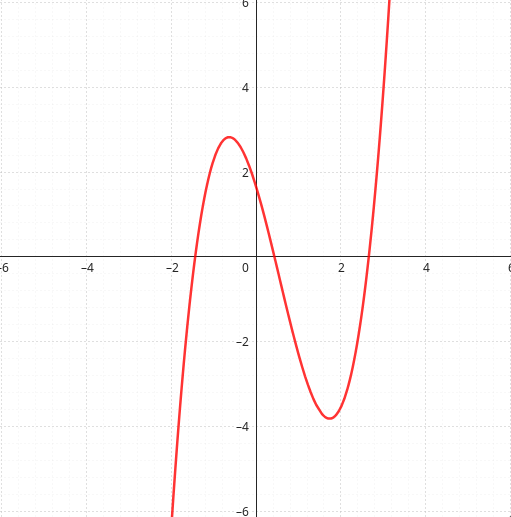
\includegraphics[width=0.6\linewidth]{Immagini/soluzione_grafica_pot_efficacie.png}
    \caption{Plot dell'equazione che descrive la derivata del potenziale efficacie: come si vede, si annulla in tre punti.}
    \label{fig:e derivata potenziale efficacie}
\end{figure}\\
Le intersezioni con il semiasse positivo delle ascisse, sono i due valori di $r$ corrispondenti al raggio di massimo avvicinamento, e l'ultima orbita stabile, o \textbf{ISCO} (Innermost stable circular orbit).
Quest'ultima, si ottiene per valori di k sufficientemente piccoli: ricordiamo che curve corrispondenti a valori di $k$ sempre più piccoli, infatti, spostano il raggio di massimo avvicinamento verso valori più alti, e abbassano il picco sempre di più, fino al limite in cui questo viene a coincidere con la valle delle orbite circolari (vedi \textbf{Figura \ref{fig:pw potential}}).  
Si noti che questa ultima orbita stabile è da considerarsi per un dato valore di $L$: quando $k\xrightarrow{}\infty$ l'ISCO tende al raggio di Schwarzschild, ma per $k$ finiti no.\\
Si noti che la \eqref{eq: derivata potenziale efficacie} presenta al suo interno una potenza cubica di $x$ e una parabola; la sottrazione delle due è rappresentata in \textbf{Figura \ref{fig:e derivata potenziale efficacie}}.
Per il valore di $k$ corrispondente all'ISCO, la tangente alla parabola e la tangente alla funzione cubica coincidono per il valore di $u$ corrispondente. 
Questo, analiticamente, si traduce nell'uguaglianza della derivata di queste due funzioni: 
\begin{figure}[h!]
    \centering
    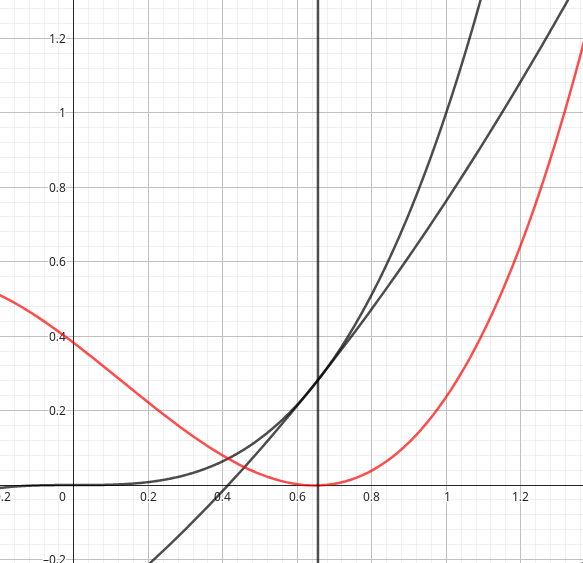
\includegraphics[width=0.5\linewidth]{Immagini/PWpot_fine_tuning.png}
    \caption{Dopo un tuning dei parametri, è stato possibile mostrare in figura la derivata del potenziale di PW come differenza della componente cubica e della parabola, nella precisa situazione in cui il minimo nel semipiano delle x positive interseca l'asse x in un punto: in corrispondenza di quel valore delle x, come si vede nella figura, la parabola e la funzione cubica hanno la tangente coincidente!}
    \label{fig:PW derivative fine tuned}
\end{figure}\\
imponendo l'uguaglianza delle derivate, e mi aspetto quindi di trovare proprio la soluzione per cui $k$ assume il valore specifico per il quale i due punti di equilibrio combaciano, come si vede in \textbf{Figura \ref{fig:PW derivative fine tuned}}.
Se nel caso di Newton il disco si spinge fino a toccare il raggio del corpo, nel caso relativistico si tronca prima, al raggio che vogliamo ora calcolare: superato questo raggio cade lungo una traiettoria a spirale che non è né chiusa, né stabile.
Non è più disco, in quanto dopo l'ISCO la velocità radiale aumenta tantissimo, e non si può più formare una regione densa: cade così velocemente che non la si può più vedere.
Dunque, seguendo quanto detto, riscriviamo la derivata del potenziale efficace, calcoliamo la derivata e mettiamo a sistema:
\begin{align}
\left\{
\begin{array}{rcl}
2u^3-(u-1)^2k^2 & = & 0 \\
u^2 - \frac{k^2}{3}u - \frac{k^2}{3} & = & 0\hspace{1mm}.
\end{array}
\right.
\end{align}
Risolvendo, con questa approssimazione, si trovano i seguenti risultati:
\begin{align}
    \left\{
    \begin{array}{rcl}
        u & = & 3 \\
        k^2 & = & 13.5\hspace{1mm},
    \end{array}
    \right.
\end{align}
mentre il risultato relativistico esatto è
\begin{align}
    \left\{
    \begin{array}{rcl}
        u_{rel} & = & 3 \\
        k^2_{rel} & = & 12\hspace{1mm}.
    \end{array}
    \right.
\end{align}
Ricordando che $u = \frac{r}{r_{sch}}$, questo significa che non ci si può avvicinare stabilmente a meno di $3$ volte il raggio di Schwarzschild (in BH di Schwarzschild).
Per buchi neri rotanti (di Kerr) si dimostra che il punto più vicino raggiungibile con un'orbita stabile è a $\frac{r_{sch}}{2}$.

\subsubsection{Discorso sull'efficienza}
Al di sotto di questi valori, il sistema cade in maniera instabile e veloce, e non può più essere considerato un sistema virializzato. 
Fino a $3 r_{sch}$ si trova
\begin{equation}
    \epsilon_{sch}=\frac{GM}{c^2r}\frac{1}{2}=\frac{GM}{c^23}\frac{1}{2}\frac{c^2}{2GM}=\frac{1}{12}
\end{equation}
per BH di Schwarzschild, mentre 
\begin{equation}
    \epsilon_{kerr} = \frac{1}{2}\frac{GM}{c^2}\frac{c^2}{GM} = \frac{1}{2}
\end{equation}
per un BH di Kerr massimamente rotante!
Se si fa accrescere la materia con il sistema "canna da pesca", si dimostra che l'efficienza è\footnote{Vedasi \cite{Rindler_Relativity}(ch. 12.2, pg. 263)}
\begin{equation}
    \epsilon_{canna}=1,
\end{equation}
mentre se la si lascia cadere radialmente senza nessuna resistenza si ha
\begin{equation}
    \epsilon_{radiale} = 0.
\end{equation}
Infine, l'accrescimento su una stella di neutroni ha efficienza pari a
\begin{equation}
    \epsilon_{NS} = \frac{GM}{c^2R}.
\end{equation}

\subsubsection{Accrescimento su NS}
La stella di neutroni è composta di materia \textit{gravitazionalmente legata}, ed è un sistema non statico ma sicuramente stazionario: è quindi virializzata.
La massa cade nella NS, e cadendo libera la sua energia senza irradiare (caduta radiale $\xrightarrow{}\epsilon=0 $: $E_{pot}=E_k$.
Nel momento in cui si scontra sulla superficie della stella, libererà sotto forma di agitazione termica esattamente metà dell'energia cinetica, in quanto a questo punto fa parte di un sistema virializzato.
La formula 
\begin{equation}
    L=\frac{GM\dot{m}}{R_{NS}},
    \label{eq: luminosità di accrescimento NS}
\end{equation}
sarebbe vera tecnicamente solo nel caso in cui tutta l'energia venisse convertita: tenendo conto di quanto appena detto, infatti, dovrebbe esserci anche un fattore $1/2$.
La soluzione di questo paradosso, sta nel fatto che per una stella di neutroni il raggio e la massa sono legati:
\begin{equation}
    R_{NS}=M^{-1/3}.   
\end{equation}
Di conseguenza, la stella di neutroni quando acquista massa si comprime un pelo, cedendo quindi energia (l'energia potenziale diminuisce, e metà di questa la libera).
Tenendo conto di questo, la formula del King, ovvero la \eqref{eq: luminosità di accrescimento NS}, è effettivamente corretta\footnote{Per il conto si veda ARTICOLO(?)}.
Per un oggetto infinitamente rigido, con indice politropico pari a $0$, effettivamente il fattore $1/2$ compare! 
Ma le stelle di neutroni \textit{pure} hanno indice politropico $3/2$.

DA COMPLETARE CON DISPENSE SE NECESSARIO
% \subsubsection{Causalità e traiettorie in Relatività}
